\documentclass[hangout,aspectratio=1610,10pt]{beamer}
%
% Choose how your presentation looks.
%
% For more themes, color themes and font themes, see:
% http://deic.uab.es/~iblanes/beamer_gallery/index_by_theme.html
%
\mode<presentation>
{
  \usetheme{NYU}      % or try Darmstadt, Madrid, Warsaw, ...
  \usecolortheme{default} % or try albatross, beaver, crane, ...
  \usefonttheme{default}  % or try serif, structurebold, ...
  \setbeamertemplate{navigation symbols}{}
  \setbeamertemplate{caption}[numbered]
} 

\usepackage{standalone}
\usepackage[english]{babel}
\usepackage[utf8x]{inputenc}
\usepackage{multirow}
\usepackage{booktabs, tabularx, colortbl}
\usepackage{changepage}
\usepackage[noplaybutton]{media9}
\usepackage[percent]{overpic}
\usepackage{hyperref}
\usepackage{attachfile2}
\usepackage{calc}
%\usepackage{subfig}
\usefonttheme[onlymath]{serif}
\usepackage{amssymb}% http://ctan.org/pkg/amssymb
\usepackage{pifont}% http://ctan.org/pkg/pifont
\newcommand{\cmark}{\ding{51}}%
\newcommand{\xmark}{\ding{55}}%
\usepackage{graphicx}
\usepackage{subcaption}
\usepackage{svg}
\usepackage{tikz}
\usepackage{bm,physics}
\usepackage{pgfplotstable}
\usetikzlibrary{tikzmark,calc,trees}
\usetikzlibrary{decorations.markings}
\usetikzlibrary{math}
\usetikzlibrary{intersections}
\usetikzlibrary{through}
\usetikzlibrary{decorations.pathreplacing,calc,decorations.markings}
\usetikzlibrary{decorations.text}
\usetikzlibrary{backgrounds}
\usepackage{color,array}
\makeatletter
\def\zapcolorreset{\let\reset@color\relax\ignorespaces}
\def\colorrows#1{\noalign{\aftergroup\zapcolorreset#1}\ignorespaces}
\makeatother
\usepackage{centernot}

\newenvironment{variableblock}[3]{%
  \setbeamercolor{block body}{#2}
  \setbeamercolor{block title}{#3}
  \begin{block}{#1}}{\end{block}}

\newenvironment{redblock}[1]{%
  \begin{variableblock}{#1}{bg=red!20,fg=black}{bg=red!80,fg=white}}{\end{variableblock}}
\newenvironment{greenblock}[1]{%
  \begin{variableblock}{#1}{bg=green!20,fg=black}{bg=green,fg=white}}{\end{variableblock}}

\newenvironment{blueblock}[1]{%
  \begin{variableblock}{#1}{bg=blue!20,fg=black}{bg=blue,fg=white}}{\end{variableblock}}
\newenvironment{yellowblock}[1]{%
  \begin{variableblock}{#1}{bg=yellow!20,fg=black}{bg=yellow,fg=white}}{\end{variableblock}}



\newenvironment{thm}[1][Theorem]{%
    \begin{variableblock}{#1}{bg=lightblue!20,fg=black}{bg=lightblue,fg=white}}{\end{variableblock}}
\newenvironment{lem}[1][Lemma]{%
    \begin{variableblock}{#1}{bg=lightblue!20,fg=black}{bg=lightblue,fg=white}}{\end{variableblock}}
\newenvironment{prop}[1][Proposition]{%
    \begin{variableblock}{#1}{bg=blue!20,fg=black}{bg=blue,fg=white}}{\end{variableblock}}
\newenvironment{defi}[1][Definition]{%
    \begin{variableblock}{#1}{bg=purple!20,fg=black}{bg=purple,fg=white}}{\end{variableblock}}
\newcommand{\bs}[1]{\textbf{#1}}
\renewcommand{\div}[1]{\text{div}{#1}}

\newcommand{\Lchild}{\mathcal{L}^{\text{child}}}
\newcommand{\Lnei}{\mathcal{L}^{\text{nei}}}
\newcommand{\Lint}{\mathcal{L}^{\text{int}}}
\newcommand{\qhat}{\hat{\vb q}}
\newcommand{\uhat}{\hat{\vb u}}
\newcommand{\q}{\vb{q}}
\newcommand{\A}{\vb{A}}
\newcommand{\Tofs}{\vb{T}^{\text{ofs}}}
\newcommand{\Tofo}{\vb{T}^{\text{ofo}}}
\newcommand{\Tifo}{\vb{T}^{\text{ifo}}}
\newcommand{\Tifi}{\vb{T}^{\text{ifi}}}
\newcommand{\Ttfi}{\vb{T}^{\text{tfi}}}
\newcommand{\CC}{\mathbb{C}}
\usepackage{forest}
\forestset{
  % Two node styles for game trees: solid and hollow
  solid node/.style={circle,draw,inner sep=1.2,fill=black},
  hollow node/.style={circle,draw,inner sep=1.2},
  % styles for long branch labels
  left label/.style={above left,midway},
  right label/.style={above right,midway},
  arrow edges/.style = for tree={{edge={<->}}},
  qtree/.style={
  align=center,}
}
\title[Application of high performance computing: earthquake hazard and infrastructure risk assessments]{Application of high performance computing: earthquake hazard and infrastructure risk assessments 
}
\author{Shanyin Tong}
\institute{Courant Institute of Mathematical Sciences, New York University}
\date{02/18/2021}
\titlegraphic{\hfill
\includegraphics[height=1.5cm]{nyu_stacked_color}}


\begin{document}

\begin{frame}
  \titlepage
\end{frame}

\begin{frame}{Earthquake hazard and infrastructure risk assessments}
\begin{columns}
\begin{column}{.6\columnwidth}
Application problem: fault-to-structure regional-scale simulations of ground motion and building response.
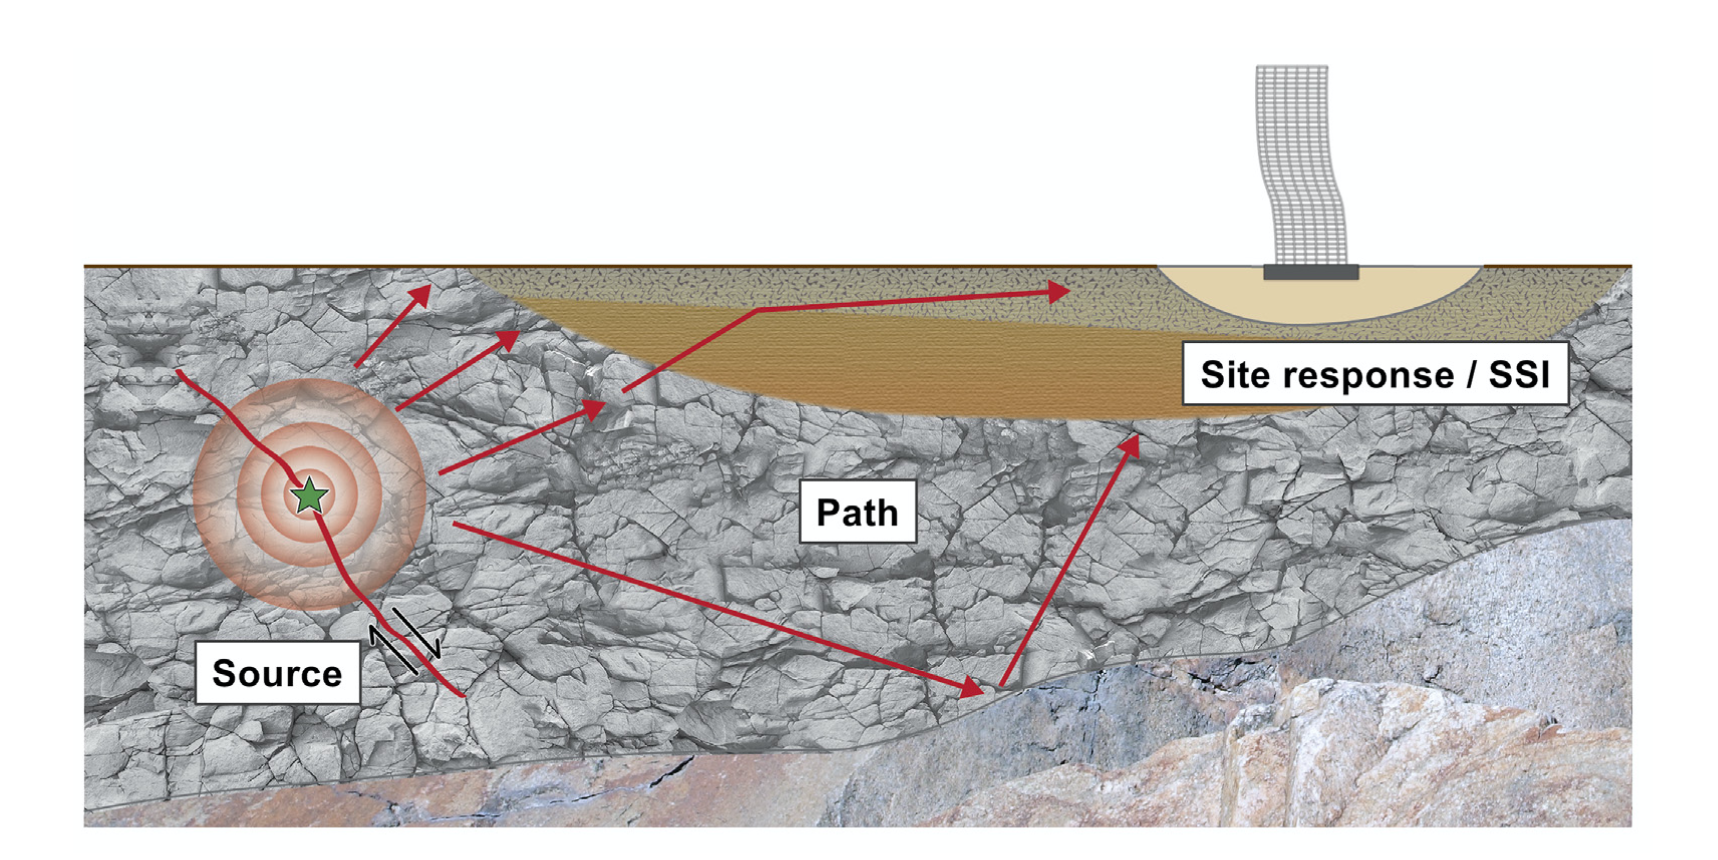
\includegraphics[width=0.9\linewidth]{plots/fig1}

Algorithms:
\begin{itemize}
	\item Earthquake ground motion simulation: SW4 (Seismic Waves, 4th order) a Summation-By-Parts (SBP) finite-difference program 
	\item Infrastructure system response: implicit, nonlinear finite element representations
\end{itemize}
\end{column}
\begin{column}{.3\columnwidth}
		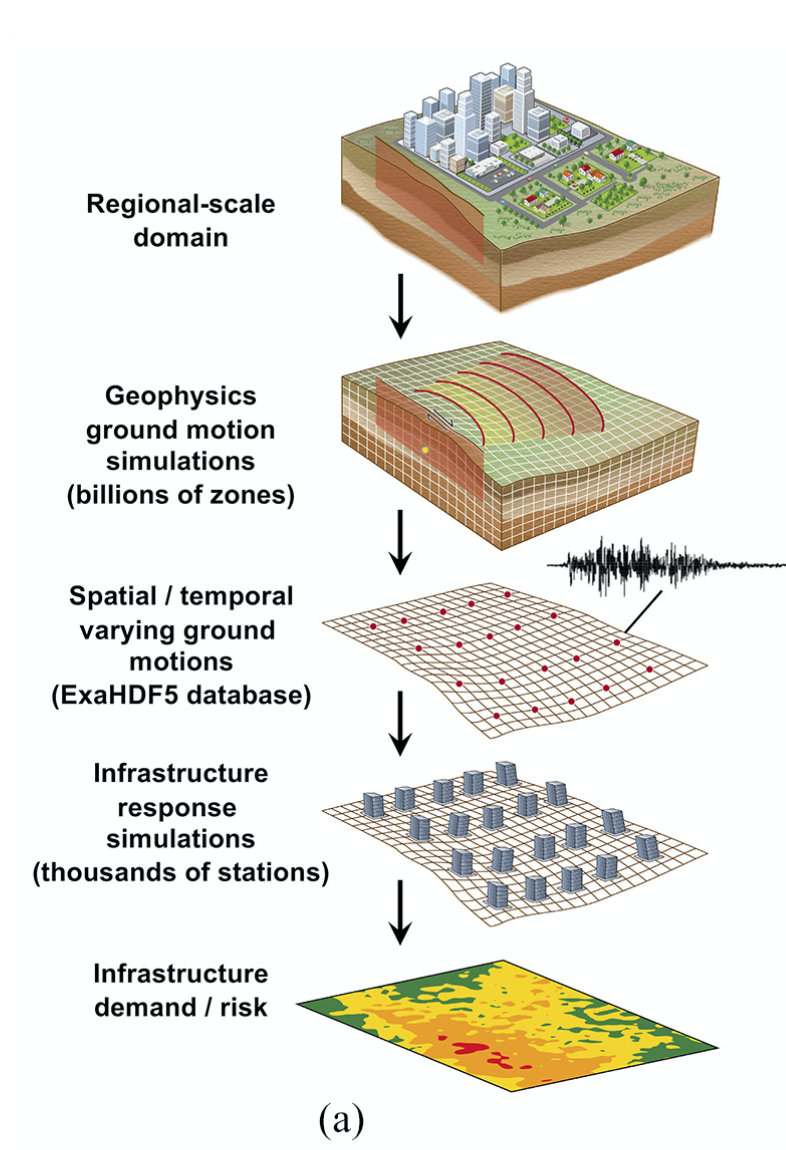
\includegraphics[width=1.2\linewidth]{plots/fig2}
\end{column}
\end{columns}
\end{frame}

\begin{frame}{High performance computing and parallel application}
\begin{columns}
	\begin{column}{.5\columnwidth}
	Super Computer:	Cori and Summit (No.2 in the the Top500 list)
		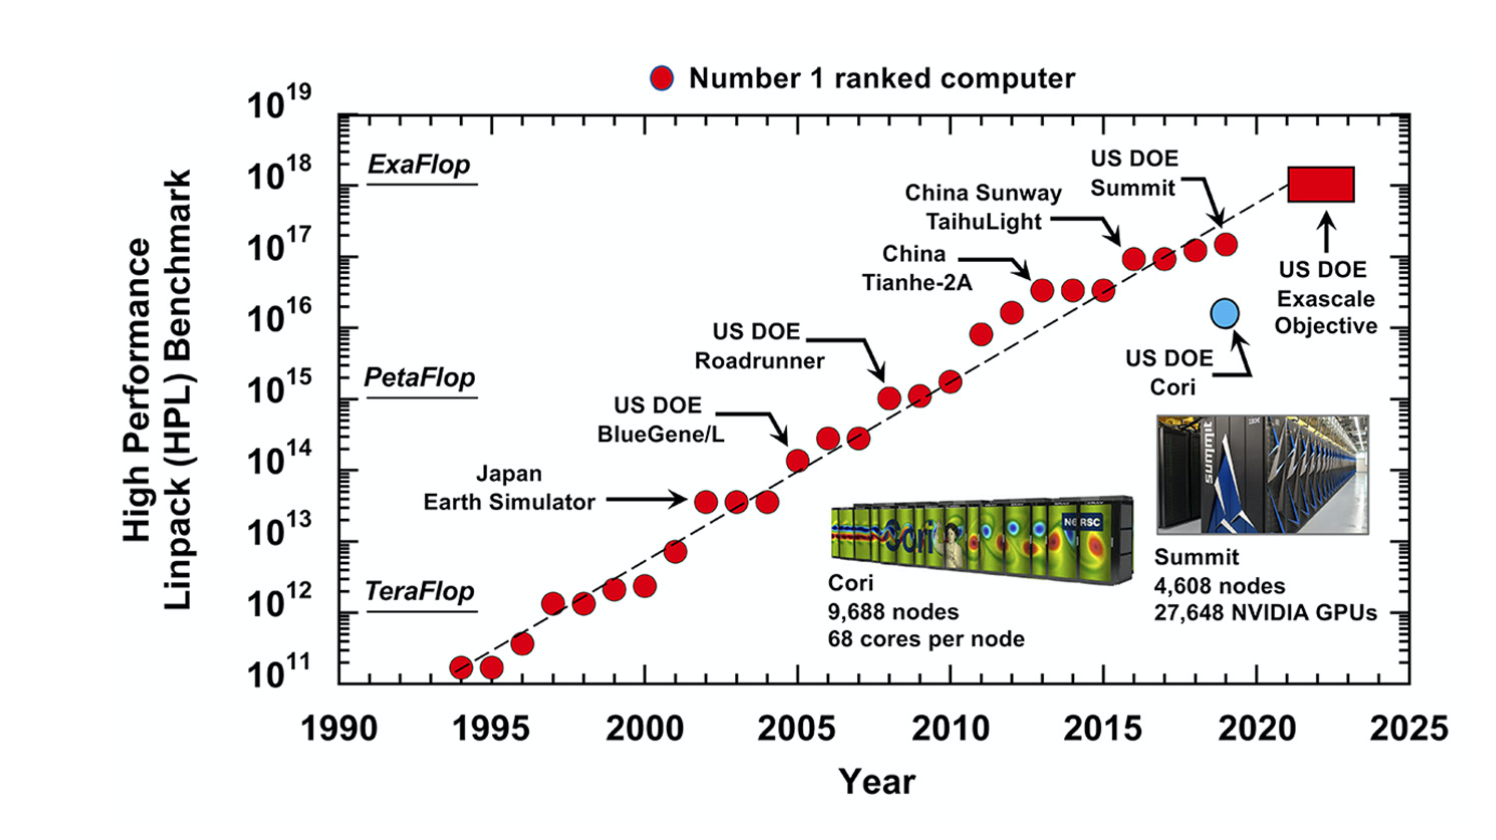
\includegraphics[width=1.\linewidth]{plots/fig3}
		
		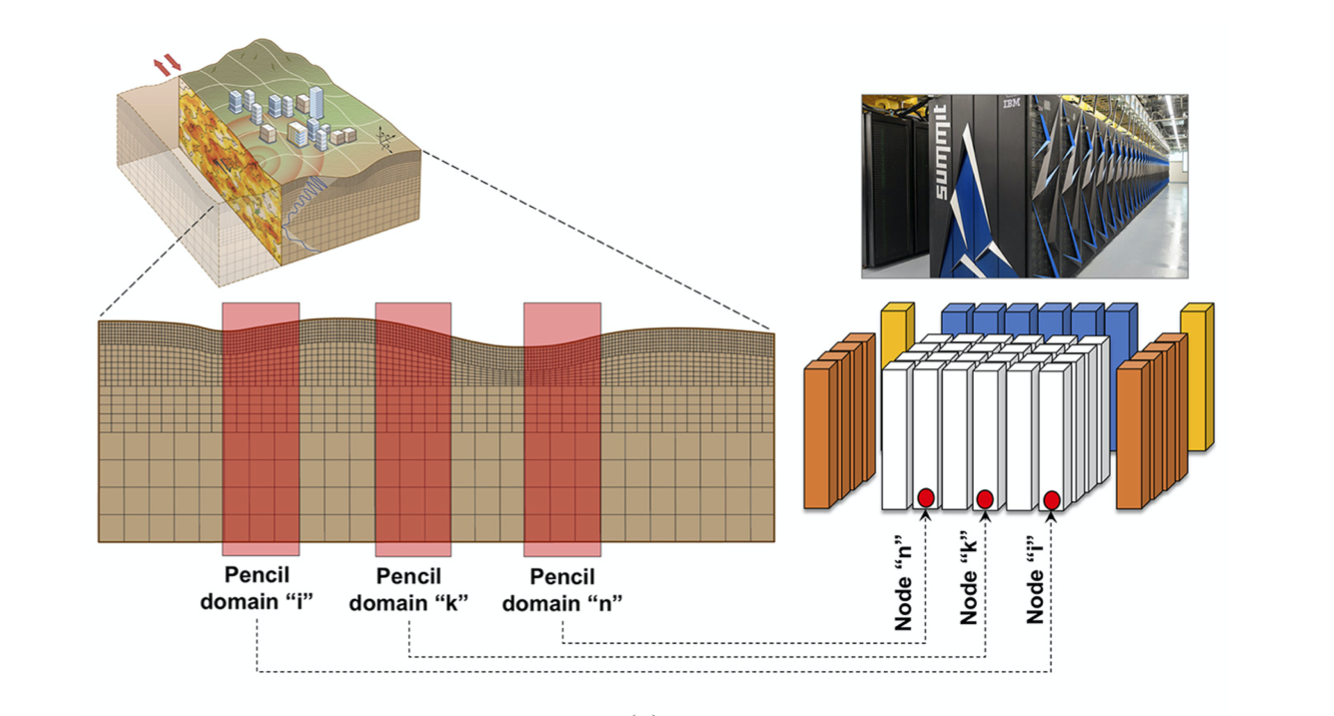
\includegraphics[width=1.\linewidth]{plots/fig12}
	\end{column}
	\begin{column}{.5\columnwidth}
		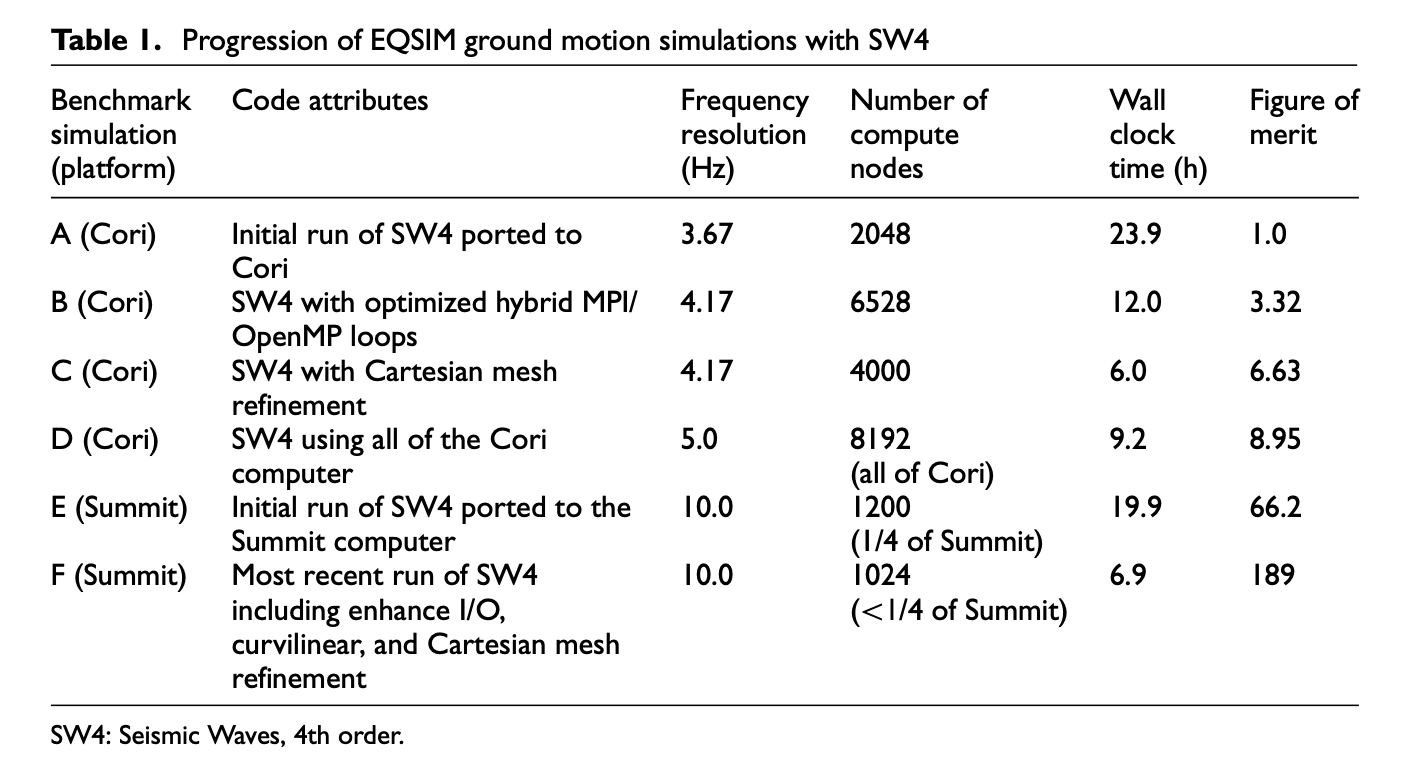
\includegraphics[width=1.\linewidth]{plots/tab1}
		
		US Department of Energy (DOE) Exascale Computing Project
		
		Top 1 computing project in National Energy Research Scientific Computing Center (NERSC)
		\vspace{10pt}
		

		\tiny{Reference: McCallen, David, et al. "EQSIM—A multidisciplinary framework for fault-to-structure earthquake simulations on exascale computers part I: Computational models and workflow." Earthquake Spectra (2020): 8755293020970982.}


		
	\end{column}
\end{columns}
\end{frame}

\end{document}